%!TEX root = ../main.tex

\chapter{Introduction\label{chap:intro}}
\minitoc
In this thesis, we focus on the unsupervised learning problem through the study of clustering in high dimensional (Gaussian) mixtures and density estimation. In this chapter, we introduce the clustering problem in the first section and the Gaussian mixtures framework in the second. In the third section, we highlight the complexities inherent to the high dimension. Then we will discuss some of the work carried out during this thesis but has been left unfinished for various reasons.
\section{Clustering and density estimation problem}
The goal of cluster analysis is to find groups in data so that each element within a group is more similar to other elements of the same group rather than to those outside of the group. The literature is rich on this topic, with different approaches coming from statistics and computer science. A clustering problem has several dimensions: the input data can be a distance or similarity matrix, the similarity can be for instance a kernel chosen by expert knowledge. The input can also be a raw data matrix with $N$ rows, the observations and $p$ columns, the features. Another dimension for clustering methods is `hard versus soft' assignment of points to clusters. In hard assignment, a point is assigned to  a unique cluster. In soft assignment, for each point, the probabilities of belonging to each clusters are furnished. This particularity is specific to probabilistic methods. A third dimension is flat versus hierarchical clustering. In flat clustering, the output is a partition of the dataset or the state-space into disjoint clusters whereas in hierarchical clustering the output is a tree of nested clusters. The latter is a finite sequence of nested partitions. We will give a glimpse on 4 well-known clustering techniques, $K$-means, Hierarchical clustering, Spectral clustering and the Gaussian mixtures model with the Expectation-Maximization algorithm (EM) which will be our topic of main interest. The reader can refer to \citep{hennig2015handbook} for an extensive review of cluster analysis.
\subsection{Centroid-Based Clustering: $K$-means}
$K$-means is a popular method of clustering which aims to partition the data into $K$ clusters such that the within-cluster sum of squares of distances to the cluster center is minimal. It has been introduced in signal theory for vector quantization by \citep{macqueen1967}. Given $N$ points, $\bx_1,\dots,\bx_N$ in $\RR^p$, the goal of $K$-means is to find a set of centers $\mathcal{C}=\{\bc_1,\dots,\bc_K\}$ that minimizes the following objective function:
\begin{equation}
  \mathcal{L}_{k\textnormal{-means}}(\mathcal{C})=\sum_{i=1}^N\min_{\bc \in \mathcal{C}}\|\bx_i - \bc \|^2.
  \label{kmeans_min_problem}
\end{equation}
Clearly this objective function is not convex and finding an exact solution of this problem is known to be NP-hard, even for $2$-means \citep{dasgupta2008hardness,Aloise:2009:NES:1519378.1519389}. As a matter of fact, for $K$ and $p$ fixed, the problem can be solved exactly in $O(n^{Kp})$ iterations \citep{Inaba:1994:AWV:177424.178042}. A simple and yet widely used approximation method to resolve the $K$-means minimization problem is Lloyd's algorithm \citep{lloyd1982}. Today, because of its popularity, Lloyd's method is assimilated with the minimization problem of $K$-means (\cref{kmeans_min_problem}). A key element of this method is the Voronoi partitioning:
\begin{defi}{(Voronoi Partition)} 
Given $n$ points in $\RR^p$, $K$ points $\bc_1,\dots,\bc_K\in \RR^p$ and a distance $d$, a Voronoi partition of $\RR^p$ consists on $K$ disjoint clusters such that for $i\in[K]$, cluster $i$ is the set of points satisfying $d(\bx, \bc_i) \leq d(\bx, \bc_j)$ for all $j\neq i$.
\end{defi}
Lloyd's procedure, depicted in \Cref{voronoi_graph} and described in \Cref{algo:lloyd_algo}, consists in building a Voronoi partition of the data from $K$ initial randomly chosen centers and iterate partitioning with the cell-means of the previous partition. The following lemma will help us to understand the convergence of the algorithm:
\begin{lemma}
Consider a finite set $\mathcal{X} \subset\RR^p$ and denote by $\bmu$ its mean. Let $d$ be a metric. For any $\by\in \RR^p$, we have that 
\begin{equation}
  \sum_{\bx \in \mathcal{X}} d(\bx,\by)^2 = \sum_{\bx\in\mathcal{X}}d(\bx,\bmu)^2 + |\mathcal{X}|d(\bmu,\by)^2.
\end{equation}
\label{lemma_lloyd_decr_cost}
\end{lemma}
The reader can refer to Fact 5.1 of \cite{hennig2015handbook} for a simple proof. This lemma claims that, after a Voronoi partitioning, replacing a center by the mean of the cell can not increase the $K$-means cost. Hence this ensures the convergence of the algorithm.
 Unfortunately, Lloyd's algorithm tends to reach local optima of the $K$-means objective. Therefore, several runs of the algorithm are necessary to ensure an acceptable clustering.
 \begin{figure}[h]
 \center
 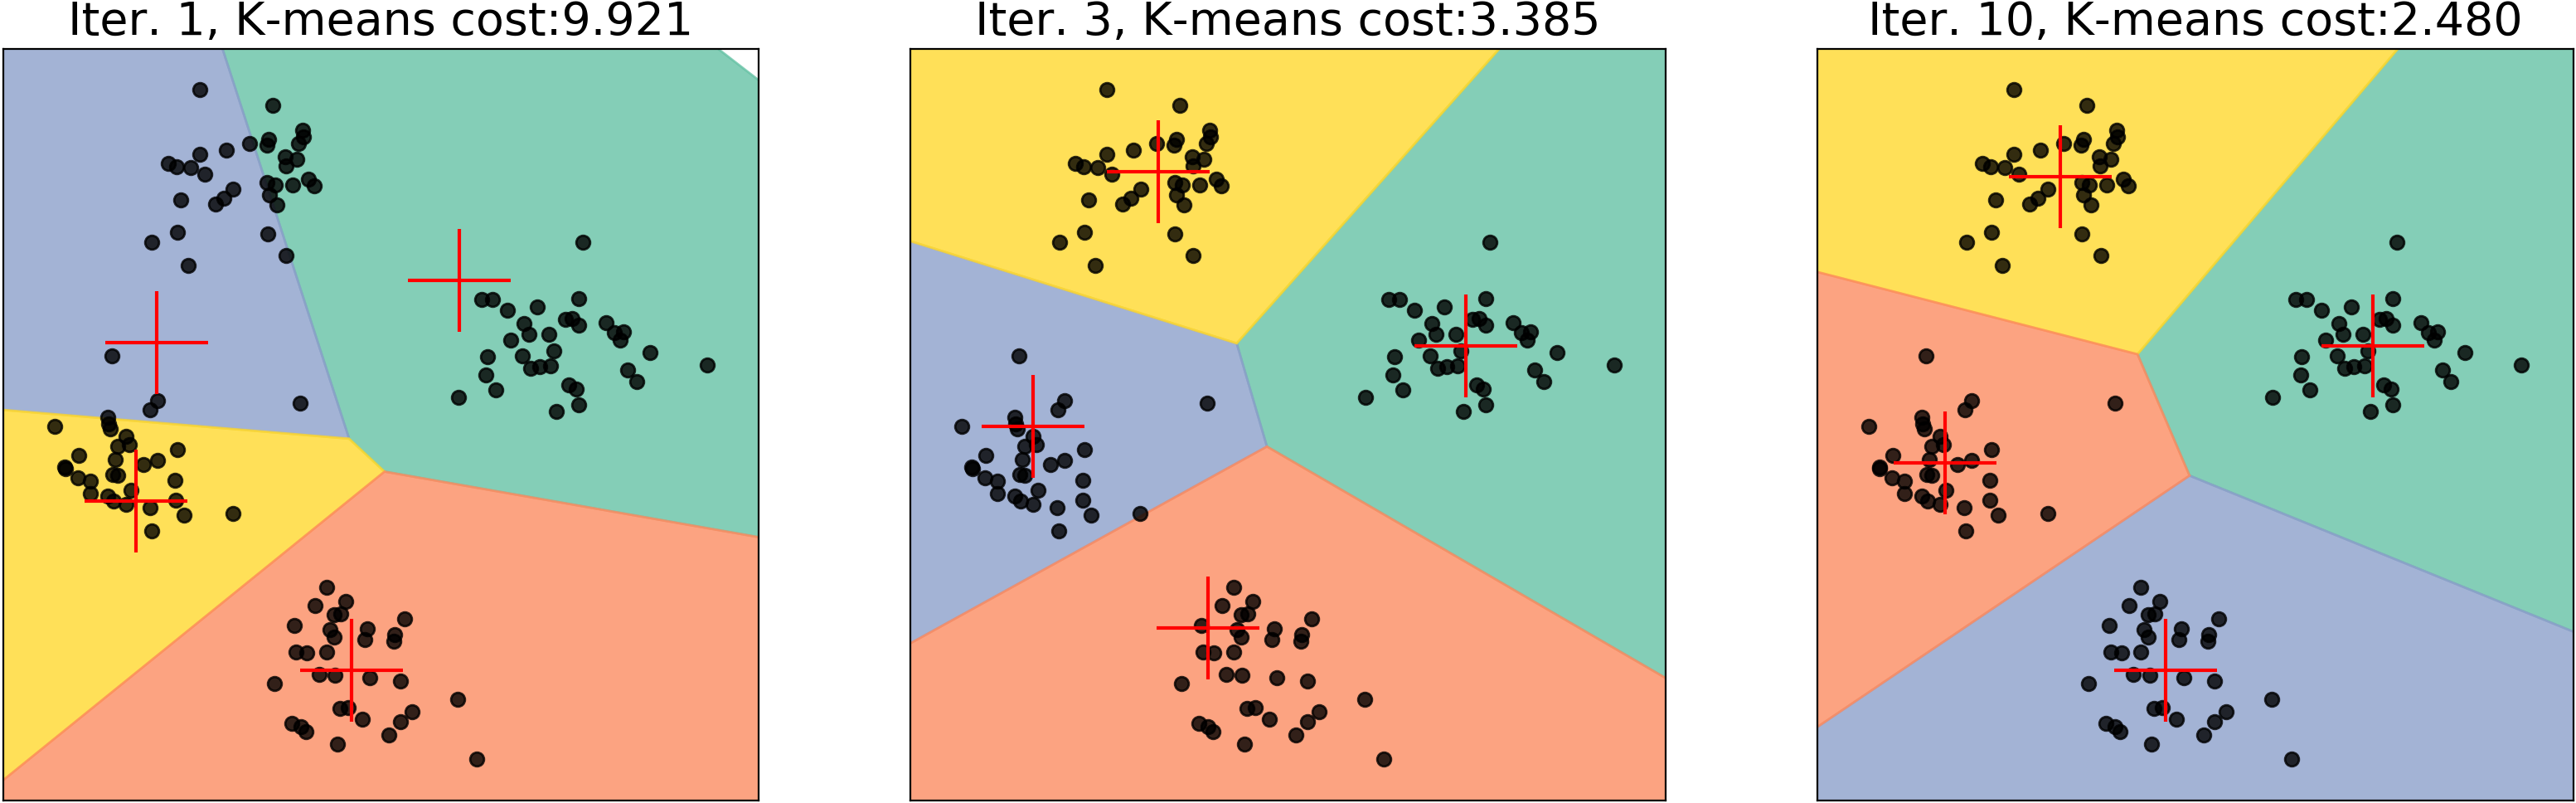
\includegraphics[scale=0.35]{TeX_files/voronoi_kmeans.png}
 \caption{Llyod's algorithm with randomly initialized centers and final Voronoi partitions at different steps: with 1 iteration (left), 3  (middle) and 10 (right) iterations (the algorithm converged). $K$-means costs are given on top.}
 \label{voronoi_graph}
 \end{figure}
\begin{figure}[h]
\begin{center}
\mybox{
\begin{minipage}{0.85\linewidth}
\begin{algorithmic}%[1]\tt
\small
\STATE {\bfseries Input:} N points $\bx_1,\ldots,\bx_N\in\RR^p$ and the number of clusters $K$.
\STATE {\bfseries Output:} Cluster centers $\hat\bc_1,\dots,\hat\bc_K$ and clusters assignments.
\STATE {\bfseries Init:} Set $\mathcal{L}_{\textnormal{old}}=\infty.$ and chose $K$ seed points $\bc_1,\dots,\bc_K$. Compute the $K$-means cost $\mathcal{L}_{\textnormal{curr}}$ given in \cref{kmeans_min_problem} with these points as centers.
\WHILE{$\mathcal{L}_{\textnormal{curr}}  < \mathcal{L}_{\textnormal{old}}$} 
\STATE{\tt 1: }Compute the Voronoi partitioning of the data with $\bc_1,\dots,\bc_K$ as centers. Get $K$ clusters, $C_1,\dots,C_K$.
\STATE{\tt 2: }For each cluster, compute the sample means $\hat\bc_1,\dots,\hat\bc_K$:
\begin{equation}
  \hat\bc_i = \frac{1}{|C_i|}\sum_{x_j\in C_i} x_j
\end{equation}
\STATE{\tt 3: }Set $\mathcal{L}_{\textnormal{old}} = \mathcal{L}_{\textnormal{curr}}$ and compute the new $K$-means cost $\mathcal{L}_{\textnormal{curr}}$ with $\hat\bc_1,\dots,\hat\bc_K$ as centers.
\ENDWHILE
\end{algorithmic}
\end{minipage}
}
   \caption{$K$-means Lloyd's algorithm}
   \label{algo:lloyd_algo}
\end{center}
\vspace{-15pt}
\end{figure}
 Note that Lloyd's algorithm has several drawbacks: 
\begin{enumerate}
\item It is a hard-assignment method since it assigns points to clusters and does not reflect a level of uncertainty on the assignments such as a probability of belonging to a cluster.
 \item The number of clusters has to be given, we will see some techniques to select the number of clusters in \Cref{estim_nb_clusters_sect}.
 \item The worst-case time complexity $T(n)$ is superpolynomial, $T(n)=2^{\Omega(\sqrt{n})}$ iterations \citep{kmeans_slow_arthur_2016} (not bounded above by any polynomial). Fortunately, in practice it is observed that Lloyd's algorithm converges quickly to a local minimum.
 \item If the initial centers are chosen randomly, the resulting $K$-means cost can be made arbitrarily bad compared to the optimal clustering (see section 5.2 of \citep{hennig2015handbook}). $K$-means$++$ \citep{Arthur:2007:KAC:1283383.1283494} addresses this problem by choosing carefully the initial centers in Lloyd's algorithm, see \Cref{algo:kmeans++_algo} for the procedure. Furthermore, $K$-means$++$ is a $\log K$ approximation algorithm for the $K$-means objective in the following sense.
\begin{theorem}{\citep{Arthur:2007:KAC:1283383.1283494}}
\label{kmeans++_theo}
Let $\mathcal{S}$ be the set of centers output by the algorithm $K$-means$++$ and $\mathcal{L}(S)$ be the $K$-means cost of the clustering obtained using $\mathcal{S}$ as the centers. Then $\EE[\mathcal{L(S)}]\leq O(\log(K))\mathcal{L}^*$, where $\mathcal{L}^*$ is the cost of the optimal $K$-means solution. 
\end{theorem}
\item $K$-means can not distinguish noise or select relevant features. This last point is particularly important in the case of high dimensional data, since it is generally accepted that the most relevant clusters lies in subspaces of much smaller dimension, we will discuss this phenomenon in \cref{curse_dim_section}. An idea would be to adapt Lloyd's method to the weighted $q^{th}$-root of the Minkowski metric
\begin{equation}
  d_{\bw}(\bx,\by) = \sum_{l=1}^p w_l|\bx_l - \by_l|^q,
\end{equation}
with $\bw$ a weight vector updated at each iterations. A first method of weighted $K$-means has been introduced in \citep{makarenkov2001optimal} and further developed in \citep{Huang_mink_kmeans} ($WK$-Means) for the Euclidean norm. An extension to the Minkowski metric ($MWK$-Means) is proposed in \citep{CordeirodeAmorim:2012:MMF:2051369.2051484} that outperforms $K$-means and $WK$-Means. Note that the use of a different metric has a profound impact on the implementation and running time since the computation of Minkowski centers is not straightforward.
\end{enumerate}
\begin{figure}[h]
\begin{center}
\mybox{
\begin{minipage}{0.85\linewidth}
\begin{algorithmic}%[1]\tt
\small
\STATE {\bfseries Input:} N points $\bx_1,\ldots,\bx_N\in\RR^p$ and the number of clusters $K$.
\STATE {\bfseries Init:} Choose one center $\bc_1$ uniformly at random among the data points and add it to the set $\mathcal{S}$.
\FOR{$j=2$ to $K$ } 
\STATE{\tt 1:} Choose a point $\bx$ from $\{\bx_1,\ldots,\bx_N\}$ with probability proportional to $\min_{\bc \in \mathcal{S}} d(\bx,\bc)^2$  and add it to $\mathcal{S}$.
\ENDFOR
\STATE {\tt 2:} Proceed with $K$-means algorithm and the set $\mathcal{S}$ as initialized centers. 
\end{algorithmic}
\end{minipage}
}
   \caption{$K$-means$++$ algorithm}
   \label{algo:kmeans++_algo}
\end{center}
\vspace{-15pt}
\end{figure}
The research on $K$-means is dense and several variants of this method has been developed. For instance $K$-medoids \citep{KaufmanR90} uses points of the data as centers, Mini-batch $K$-means \citep{Sculley:2010:WKC:1772690.1772862} takes mini-batches of data to reduce significantly computational cost without penalizing too much the $K$-means cost, or clustering algorithms that enjoy strong theoretical guarantees on non-worst case scenarios using the notion of stability \citep{Ostrovsky2006}. The reader can refer to \citep{hennig2015handbook} for further details on this topic.

\subsection{Agglomerative Hierarchical Methods}
In this section, we will present the Agglomerative Hierarchical clustering, a very popular method due to its simplicity and the nested structure of clusters that it produces. The idea of Hierarchical clustering is to form a hierarchy of clusters (\textit{i.e.} nested partitions) according to a merging rule which helps us to see how clusters are related to each other (a structure unavailable with the other methods). There exist two types of hierarchical clustering: agglomerative and divisive. The first type consists in starting from $N$ clusters, each containing one element of the dataset and in merging clusters iteratively into larger groups according to an agglomeration rule and a similarity. This process builds a hierarchy, until finding only one cluster that contains the whole dataset. The similarity can be a Minkowski distance, the cosine similarity or other distance such as Hamming, Hellinger or Mahalanobis.  The divisive procedure is the opposite of the agglomerative: starting from the whole dataset and splitting iteratively until obtaining $N$ clusters. Divisive methods are generally very expensive, with a complexity of $O(2^n)$ \citep{Guenoche1991}, and are therefore not used in practice. 
Let us consider the agglomerative procedure and a metric $d$, a simple implementation is to build the dissimilarity matrix of the $N$ original clusters $\{\bx_1\},\dots,\{\bx_N\}$ noted $S=(d_{ij}=d(\bx_i,\bx_j))_{i,j\in [N]^2}$ (which is symmetric) and consider the couple $(i,j)$ such that $d_{ij}$ is the smallest dissimilarity in $S$. We create a new cluster $i \cup j$, add it to the matrix $S$ with the rule $d_{i\cup j, k}=\min\{d_{ik},d_{jk}\}$ and remove the rows and columns of sets $i$ and $j$ from $S$. The iteration of this procedure leads to one final cluster containing all points in the dataset. This method is called `Single-linkage' clustering \citep{Graham:1985:HMS:1435654.1436662}; a naive implementation of it with a complexity of $O(n^3)$ is given in \Cref{algo:single_linkage_hier_algo}. Note that it can be optimized to $O(n^2)$\citep{hierarchicalMurtagh}. The hierarchy can be visualized via a binary tree called ``dendrogram'', see an illustration in \Cref{dendrogram_graph}. This method has a severe drawback called `chaining phenomenon' referring to the fact that clusters can be merged due to the presence of close points even if they contain other points that are very distant. An alternative method called `Complete-linkage' clustering solves this problem by taking the maximum instead of the minimum in step 1 of the Single-linkage algorithm in \Cref{algo:single_linkage_hier_algo}. Similarly to Single-linkage method, the complexity of the naive implementation is $O(n^3)$ but can be optimized to $O(n^2)$. Another popular method worth mentioning for its use of cluster centers is Ward's method\citep{ward63} also called Ward's minimum variance method which consists in optimizing an objective function, generally the sum of squared Euclidean distances between points. Let us consider the merging cost of combining clusters $A$ and $B$. If $A\cap B = \emptyset$, then
\begin{align*}
  \Delta(A,B) &= \sum_{i\in A\cup B} \|\bx_i - \bc_{A \cup B} \|^2-\sum_{i\in A} \|\bx_i - \bc_{A} \|^2-\sum_{i\in B} \|\bx_i - \bc_{B} \|^2\\
  &= \frac{n_An_B}{n_A+ n_B}\|\bc_A - \bc_B \|^2,
\end{align*}
where $\bc_I$ and $n_I$ are the center of cluster $I$ and its size respectively.  This quantity is positive, hence the within-group variance increases when merging two clusters. Ward's method seek to minimize this growth. Alternatively, this amounts to looking for the maximum between-cluster variance. 

We can notice that agglomerative methods might differ on the computation of dissimilarities following the agglomeration process (step 2 in \Cref{algo:single_linkage_hier_algo}). Lance and Williams developed an updating formula \citep{lance_williams_67} for these dissimilarities that generalizes several agglomerative methods. The dissimilarity between a new merged cluster $i \cup j$ and cluster $k$ is
\begin{equation}
  d(i \cup j,k) = \alpha_i d(i,k)+\alpha_jd(j,k)+\beta d(i, j) +\gamma |d(i,k)-d(j,k)|,
\end{equation}
where the parameters $\alpha_i , \alpha_j, \beta, \gamma$ depend on the clustering criterion. For instance, the single-linkage method is recovered by setting $\alpha_i =\alpha_j = 1/2$, $\beta =0$ and $\gamma =-1/2$, the complete-linkage method with $\alpha_i =\alpha_j = 1/2$, $\beta =0$ and $\gamma =1/2$ and Ward's method can be expressed in this framework \citep{Batagelj88generalizedward,f.1985multidimensional,jambu1989exploration} with $\alpha_i=(n_i+n_k)/(n_i+n_j+n_k)$, $\alpha_j=(n_j+n_k)/(n_i+n_j+n_k)$, $\beta=-n_k/(n_i+n_j+n_k)$ and $\gamma=0$. The reader can find parameters for other methods in Table 6.1 of \citep{hennig2015handbook}.
 \begin{figure}[h]
 \center
 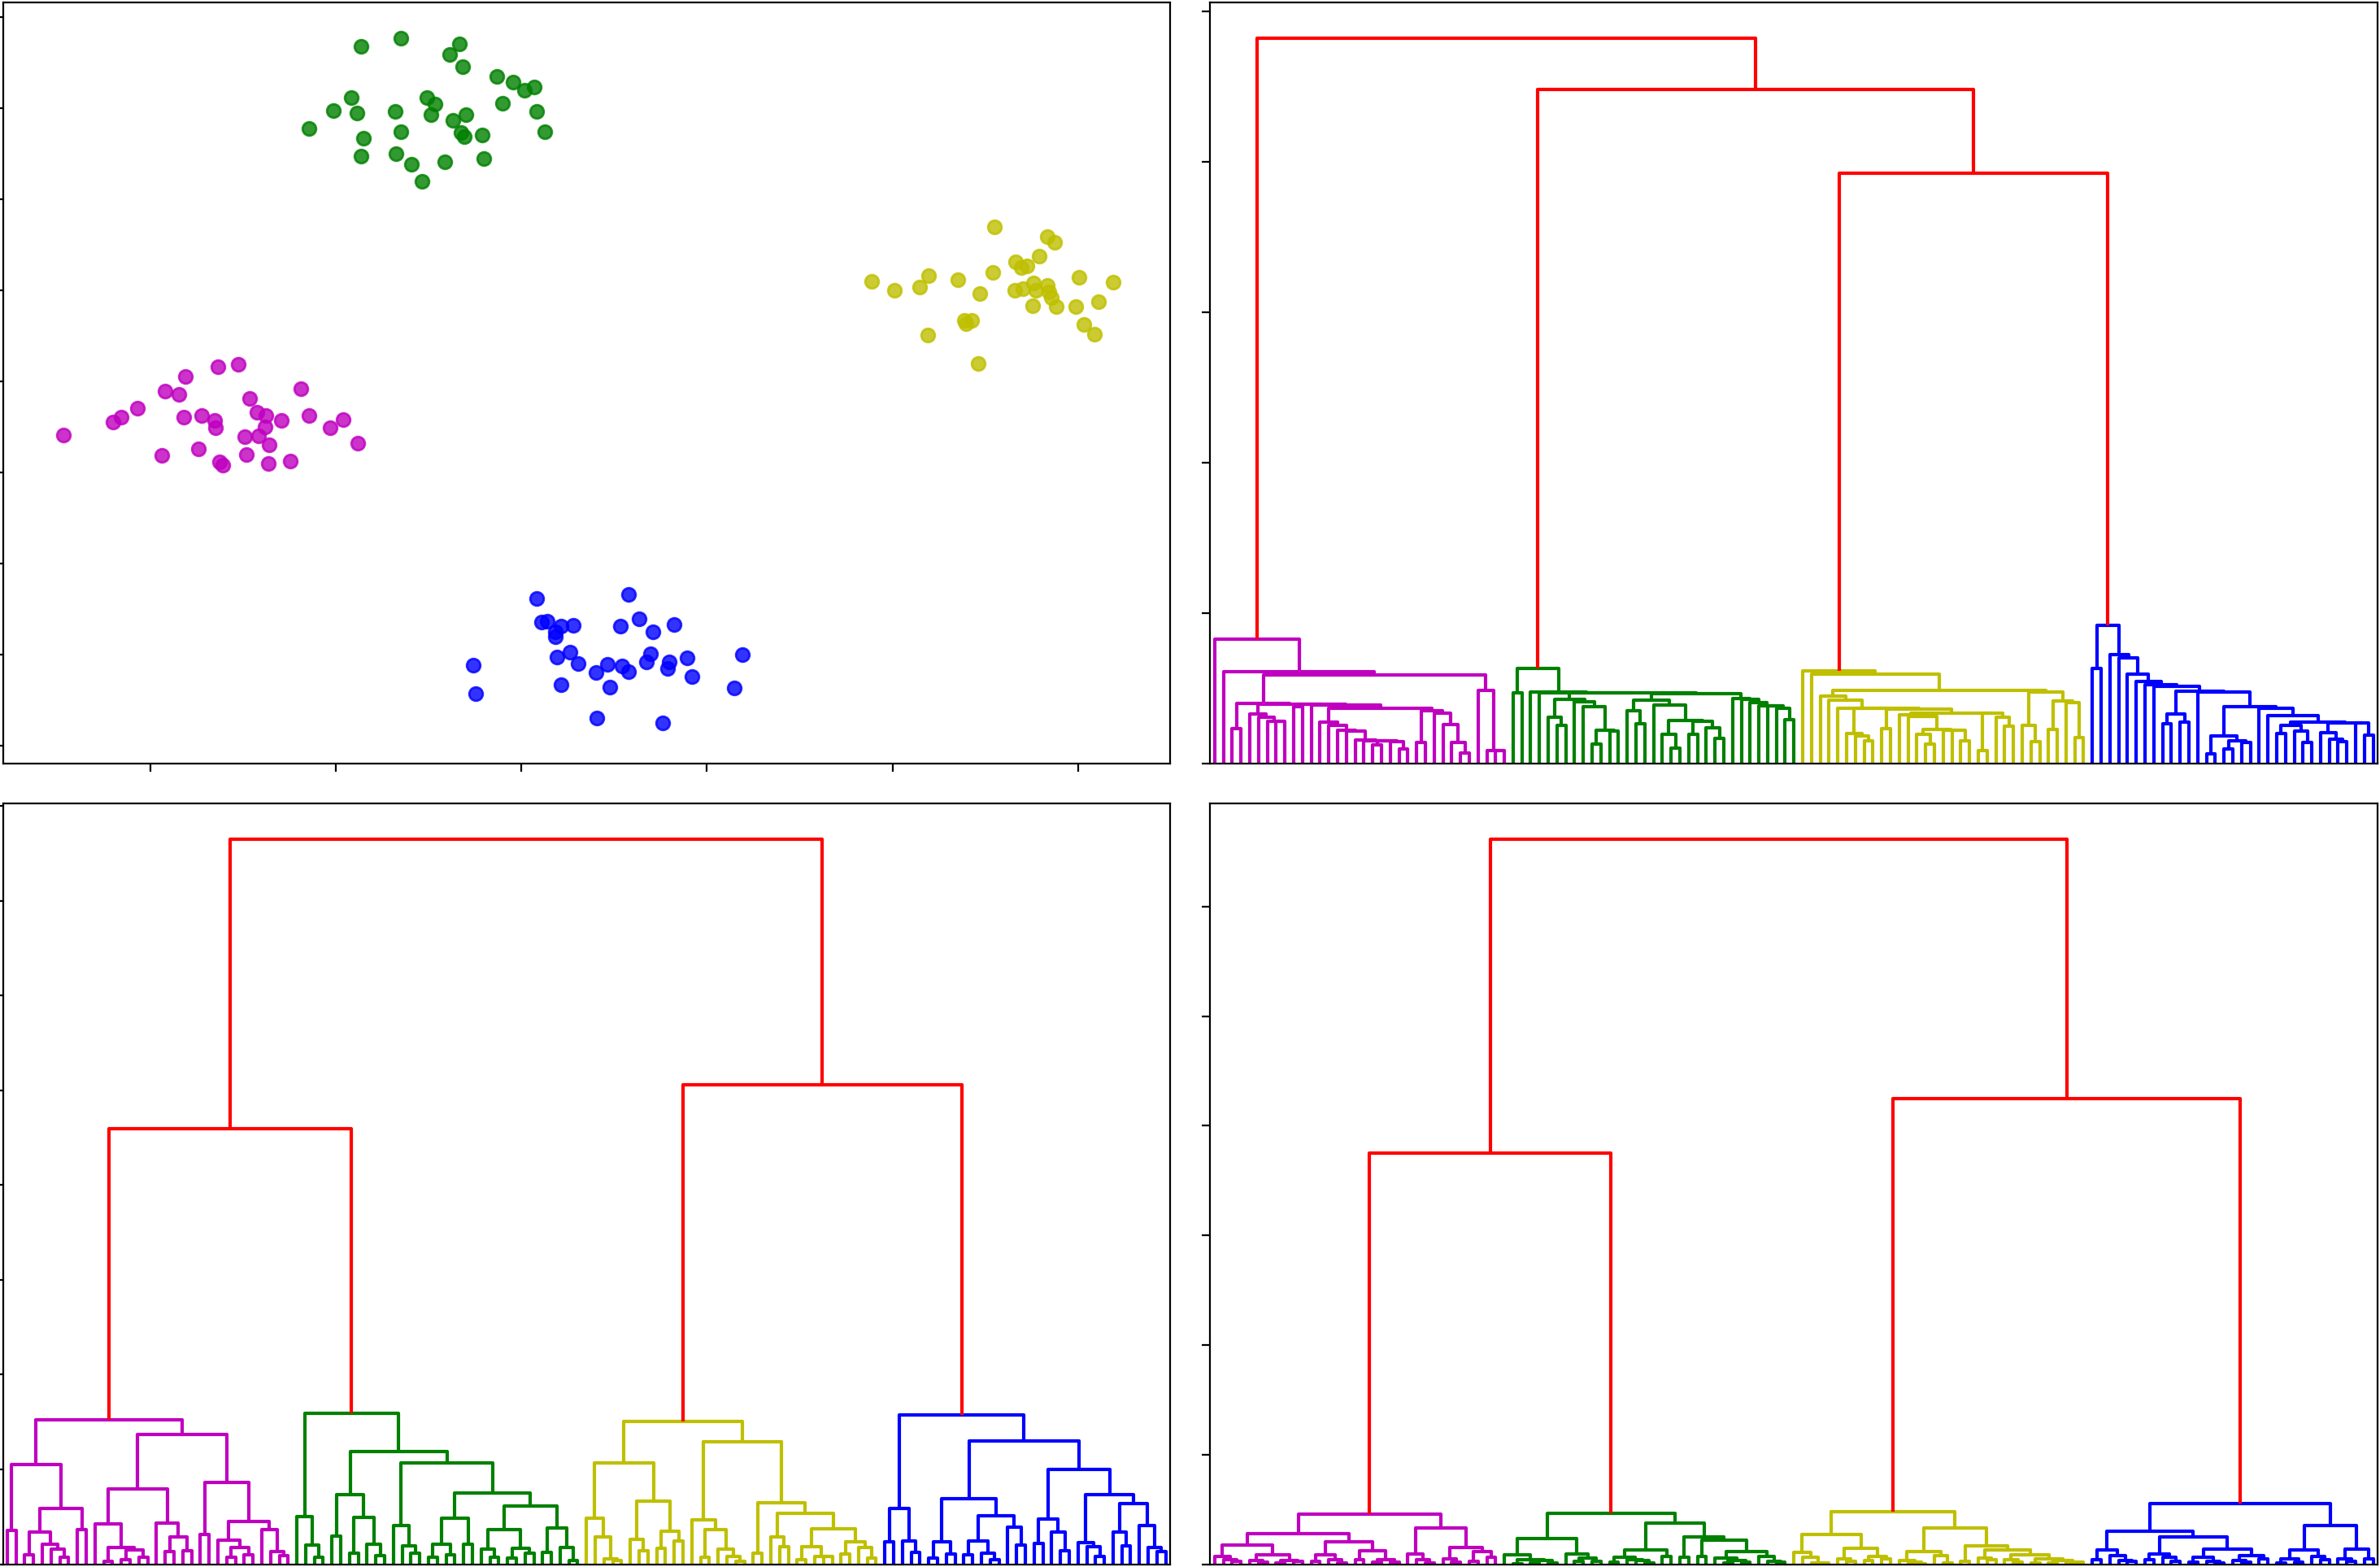
\includegraphics[scale=0.35]{TeX_files/dendrogram.png}
 \caption{A dataset with 4 clusters (top-left) used with the Agglomerative hierarchical clustering and the corresponding dendrogram, single-link (top-right), complete-link (bottom-left) and Ward's method (bottom-right). A simple way for finding clusters would be to cut the dendrogram with a horizontal line from bottom to top until finding the number of clusters desired. Note the difficulty to recover the 4 original clusters.}
 \label{dendrogram_graph}
 \end{figure}
 More efficient algorithms rely on `Nearest Neighbor Chains'. We invite the reader to refer to \citep{hierarchicalMurtagh} for a detailed review on Agglomerative hierarchical methods.

\begin{figure}[h]
\begin{center}
\mybox{
\begin{minipage}{0.85\linewidth}
\begin{algorithmic}%[1]\tt
\small
\STATE {\bfseries Input:} A similarity matrix $S$.
\WHILE{at least 2 objects remain in S} 
\STATE{\tt 1:} Determine the smallest dissimilarity $d_{ij}$ in $S$.
\STATE{\tt 2:} Let $m$ be the size of $S$, compute the dissimilarities for the new cluster $i\cup j$:
\begin{equation}
  d_{i\cup j, k} = \min\{d_{ik},d_{jk}\},\quad k\in [m], k\neq i,j.
\end{equation}
\STATE{\tt 3:} Add the dissimilarities of $i\cup j$ in $S$ and remove those of clusters $i$ and $j$.
\ENDWHILE
\end{algorithmic}
\end{minipage}
}
   \caption{Simple single-linkage hierarchical clustering}
   \label{algo:single_linkage_hier_algo}
\end{center}
\vspace{-15pt}
\end{figure}
\subsection{Spectral clustering}
Recently, spectral clustering has become widely used thanks to its performance compared to traditional clustering techniques and its computational attractiveness. One interesting feature of spectral clustering is that it does not make any assumption on the form of the clusters contrary to $K$-means. This method of clustering relies deeply on the graph theory \citep{Donath:1973:LBP:1664638.1664644,Fiedler1973}. The reader can refer to \citep{Luxburg:2007:TSC:1288822.1288832} and \citep{SPIELMAN2007284} for a survey of the literature on this topic. Although several methods exist which all are referred to as ``Spectral clustering'' we will describe the simplest formulation of this method. Let us consider $\bx_1,\dots,\bx_N$, $N$ points in $\RR^p$ and a similarity measure $s_{ij} \geq 0$ between $\bx_i$ and $\bx_j$. We can construct the similarity matrix $\bS=(s_{ij})_{i,j\in [N^2]}$ which can be represented by a similarity graph $G=(V,E)$ where the vertices $v_1,\dots,v_N$ correspond to the points $\bx_1,\dots,\bx_N$ and the edge between $v_i$ and $v_j$ exists if $s_{ij}\neq 0 $ and thus has weight $s_{ij}$. Note that $G$ is an undirected graph, \textit{i.e.} $s_{ij}=s_{ji}$. The main idea of spectral clustering is to find a partition of $G$ with minimal cuts, that is to find a partition such that the cumulative weight of the edges between different groups is low and those within a group are high. This can be done by analyzing the spectrum of the Laplacian matrix $\bL$ of $\bS$ and a clustering such as $K$-means in a low-dimensional subspace spanned by eigenvectors of $\bL$ corresponding to its largest eigenvalues. It is clear that a sparse graph $G$ is interesting for such a cutting problem. There exist several methods to sparsify $\bS$:
\begin{description}
\item[$K$-nearest neighbor graphs:] Modify the similarity matrix $\bS$ by keeping for each nodes the $k$-nearest neighbors and set $s_{ij}=0$ for the other vertices. We can make this graph undirected in different ways, see section 2.2 of \citep{Luxburg:2007:TSC:1288822.1288832}.
\item[$\varepsilon$-neighborhood graph:] We connect nodes $v_i$ and $v_j$ if $s_{i,j}\geq \varepsilon$, this graph is usually unweighted.
\end{description}
We will note $\bW$ the resulting weighted adjacency matrix. The reader can find more details on the behavior of these different graphs in section 8 of \citep{Luxburg:2007:TSC:1288822.1288832}. The simplest approach for spectral clustering is to consider the `unnormalized graph Laplacian', $\bL=\bD-\bW$, where $\bD$ is a diagonal matrix called the `degree matrix' and the element $i$ of its diagonal is the degree of the vertex $v_i$, $d_i= \sum_{j=1}^Ns_{ij}$. An important property of this matrix is that its smallest eigenvalue is 0 and the corresponding eigenvector is the constant vector (see Proposition 1 of \citep{Luxburg:2007:TSC:1288822.1288832}). In the sequel, we say that $A \subset G$ is connected if any two vertices in $A$ can be joined with a path such that all the intermediate vertices lie in $A$. The subgraph $A$ is a connected component if it is connected and there are no connections between $A$ and its complement $\bar A$. An important result for spectral clustering is the following proposition:
\begin{proposition}[Number of connected components, proposition 2 in \citep{Luxburg:2007:TSC:1288822.1288832}]
 The multiplicity $k$ of the eigenvalue 0 of $\bL$ is the number of connected components $A_1,\dots,A_k$ in the graph $G$. The eigenspace of eigenvalue 0 is spanned by the indicator vectors $1_{A_1},\dots,1_{A_k}$ of these components.
 \end{proposition}
 The simplest implementation of the spectral clustering is given in \Cref{algo:unnorm_spectr_alg}.
 \begin{figure}[h]
\begin{center}
\mybox{
\begin{minipage}{0.85\linewidth}
\begin{algorithmic}%[1]\tt
\small
\STATE {\bfseries Input:} A similarity matrix $\bS\in \RR^{N\times N}$ and the number of clusters to find $k$.
\STATE {\bfseries Output:} Clusters $A_1,\dots,A_k$.
\STATE{\tt 1:} Construct the weighted adjacency matrix $\bW$.
\STATE{\tt 2:} Compute the unnormalized Laplacian $\bL$.
\STATE{\tt 3:} Compute the $k$ eigenvectors $\bv_1,\dots,\bv_k$ of $\bL$ corresponding to the $k$ smallest eigenvalues of $\bL$.
\STATE{\tt 4:} Let $\bV\in \RR^{N\times k}$ be the matrix containing the vectors  $\bv_1,\dots,\bv_k$  as columns.
\STATE{\tt 5:} For $i \in [N]$, let $\by_i \in \RR^k$ be the vector corresponding to the $i^{th}$ row of $\bV$.
\STATE{\tt 6:} Cluster the points $(\by_i)_{i\in[N]} \in \RR^k$ with the $k$-means algorithm into clusters $C_1,\dots,C_k$.
\STATE{\tt 7:} Construct clusters $A_1,\dots,A_k$ with $A_i=\{i, \by_i \in C_i\}$
\end{algorithmic}
\end{minipage}
}
   \caption{Unnormalized spectral clustering according to \citep{Luxburg:2007:TSC:1288822.1288832}}
   \label{algo:unnorm_spectr_alg}
\end{center}
\vspace{-15pt}
\end{figure}
Two other types of Laplacian matrices are used in the literature called ``normalized graph Laplacians'' and offer theoretical advantages compared to the unnormalized Laplacian (see section 8.4 of \citep{Luxburg:2007:TSC:1288822.1288832}). They are defined as follows:
\begin{equation}
  \bL_{\textnormal{sym}} = \bI - \bD^{-\nicefrac{1}{2}}\bW\bD^{\nicefrac{1}{2}} \quad \textnormal{and} \quad \bL_{\textnormal{rw}}= \bI-\bD^{-1}\bW.
\end{equation}
We will refrain from addressing these two matrices, we shall content ourselves with saying that there exist more efficient spectral clustering algorithms called ``Normalized spectral clustering'' that are of the same spirit as \Cref{algo:unnorm_spectr_alg}, the reader can refer to \citep{Shi:2000:NCI:351581.351611,Ng01onspectral,Luxburg:2007:TSC:1288822.1288832} for a deeper analysis of the use of these Laplacians. We will simply give an insight on the mechanics behind the spectral clustering algorithm and we shall highlight the problem from a graph point of view. The spectral algorithm is an approximation to the problem of partitioning the graph $G$. For $A$ and $B$, two disjoint subsets of the vertex set $V$ of $G$ we define the cut of $A$ and $B$ as:
\begin{equation}
  cut(A,B)=\sum_{i\in A, j\in B} w_{ij}.
\end{equation}
Two common objective functions to minimize for such partitioning are RatioCut \citep{Hegen1992} and Ncut \citep{Shi:2000:NCI:351581.351611} defined as 
\begin{align*}
&\textnormal{RatioCut}(A_1,\dots,A_k)=\sum_{i=1}^k\frac{cut(A_i,\bar A_i)}{|A_i|},\\
&\textnormal{Ncut}(A_1,\dots,A_k)=\sum_{i=1}^k\frac{cut(A_i,\bar A_i)}{\textnormal{vol}(A_i)},
\end{align*}
where $|A|$ is the number of vertices in $A$ and $\textnormal{vol}(A) = \sum_{i\in A}d_i$. Note that these two objective functions try to achieve a "balanced" partitioning, a small component leads to a high value of these objective functions. Unfortunately, solving such a partitioning problem is NP-hard \citep{Wagner1993,Luxburg:2007:TSC:1288822.1288832}. Fortunately, a relaxation of this problem with RatioCut is:
\begin{equation}
\label{relaxed_ratiocut_pb}
  \min_{\bH\in{\RR^{N\times K}}} Tr(\bH^T\bL\bH)\quad \textnormal{subject to}\quad \bH^T\bH = \bI,
\end{equation}
and can be solved explicitly. It turns out that choosing $\bH$ as the matrix with the first $k$ eigenvectors of $\bL$ as columns is a solution of \Cref{relaxed_ratiocut_pb} (see 5.2 of \citep{Luxburg:2007:TSC:1288822.1288832}) which is exactly step 4 in \Cref{algo:unnorm_spectr_alg}. Similar relaxation can be done for the Ncut objective function
\begin{equation}
  \min_{\bU\in\RR^{N\times k}} Tr(\bU^T\bD^{-\nicefrac{1}{2}}\bL\bD^{-\nicefrac{1}{2}}\bU)\quad \textnormal{subject to}\quad \bU^T\bU = \bI.
\end{equation}
These relaxations do not give guarantees on the quality of the solutions and the resulting partition can be significantly worse than the optimal one in regards to RatioCut and Ncut \citep{Guattery98,Nadler07fundamentallimitations}. In particular, spectral clustering methods are global methods and fail to identify clusters at different scales \citep{Nadler07fundamentallimitations}. But these approximations are computationally attractive and very simple to solve, especially with a sparse weighted adjacency matrix.

\subsection{Finding the number of clusters}\label{sec:estim_nb_clusters}
\label{sec:finding_clusters_nb}
The determination of the number of clusters in a dataset is fundamental and still unsolved problem. Numerous approaches to this problem has been developed over the years, see \citep{Hardy:1996:NC:255810.255820,Milligan1985} and Chapter 26 of \citep{hennig2015handbook}. Several popular heuristics rely on a graphical interpretation of the quality of clustering. The most popular is the Elbow criterion which consists in performing clusterings with different number of clusters $K$ and computing the ratio of the between group variance and the total variance (the F-test statistic) for each $K$. The detection of an `elbow' indicates the appropriate number of clusters; \textit{i.e.} clusterings with larger $K$ do not really improve the explained proportion of the variance. Another technique that relies on a graphical interpretation is the Silhouette method \citep{Rousseeuw:1987:SGA:38768.38772} which assesses how well a point is assigned to its cluster compared to nearest neighbor cluster. A more formal approach is the `Gap Statistic' developed in \citep{gap_stat_tibsh_2001}, an efficient statistical procedure that compares the change in within-cluster dispersion with that expected under a reference null distribution. In the case of the spectral clustering, one can use the `eigengap' heuristic on the eigenvalues $\lambda_1,\dots,\lambda_N$ of the Laplacian matrix by choosing $K$ such that $\lambda_1,\dots,\lambda_K$ are small and $\lambda_{K+1}$ is relatively large (see section 8.3 of \citep{Luxburg:2007:TSC:1288822.1288832}). Finally, a model selection criterion widely used in probabilistic models and important in our work is the Bayesian Information Criterion (BIC). This method has been developed in \citep{schwarz1978} following the work of Akaike on the AIC \citep{Akaike1998}. The idea of this method, under the assumption that the observations $\{\bx_1,\dots,\bx_N\}$ are drawn from an exponential family, is to derive from the approximation of the asymptotic expansion of the Bayes estimator the following quantity
\begin{equation}
  \textnormal{BIC} = \hat\ell_j(\hat\theta_j,\bx)-\frac{1}{2}k_j\log(N),
\end{equation}
where $\hat\ell_j(\hat\theta,\bx)$ is the maximized log-likelihood of model $j$, $\hat\theta_j$ is the MLE and $k_j$ is the number of free parameters of model $j$. Therefore, the model selection rule is to choose the model for which the BIC is the largest. BIC has several nice properties; in particular, it penalizes the complexity of the model which is interesting since choosing the model only on the criterion of the{} likelihood in the case of Gaussian mixtures leads to select as many components as there are points. 

One can remark that all procedures mentioned previously require to perform a large number of clusterings and select the best model according to a given criterion. Such an approach is computationally expensive. In \Cref{sparse_weight_vect_estim}, we try to address this challenge by iteratively penalizing the weight vector of large Gaussian mixture in an EM-like procedure.

\section{The Gaussian Mixture Model}
We will now focus on the Gaussian Mixture Model (GMM), an important framework for clustering problems. Unlike the other previously seen methods, it is a probabilistic approach to clustering. One of the main advantages of model-based clustering is that the resulting partition can be interpreted statistically. It assumes that the observations are drawn from a
mixture distribution the components of which are Gaussian  with parameters $(\bmu_k,\bSigma_k)$, the density of the $k$-th mixture component is
\begin{equation}
\varphi_{\bmu_k,\bSigma_k}(x)=\frac{1}{(2\pi)^{p/2}|\bSigma_k|^{1/2}} \exp\Big(-\frac{1}{2}(\bx-\bmu_k)^\top\bSigma_k^{-1}(\bx-\bmu_k)\Big).
\end{equation}
Let $\btheta$ be the list containing all the unknown parameters of a Gaussian mixture model: the family of means $\bmu = (\bmu_1,\ldots,\bmu_K)
\in (\RR^p)^K$, the family of covariance matrices $\bSigma = (\bSigma_1,\ldots,\bSigma_k)\in(\mathcal S_{++}^p)^K$ and the vector of cluster probabilities  $\bpi=(\pi_1,\ldots,\pi_K)\in [0,1]^K$ such that $\b1_K^\top\bpi=1$.
The density of one observation $\bX_1$ is then given by:
\begin{equation}\label{mixture}
p_{\btheta}(\bx)=\sum_{k=1}^K\pi_k\varphi_{\bmu_k,\bSigma_k}(\bx),\qquad \forall \bx\in\RR^p,
\end{equation}
where $\btheta=(\bmu,\bSigma,\bpi)$.
This model can be interpreted from a latent variable perspective. Let $Z$ be a discrete random variable
taking its values in the set $[K]$ and such that $\Pb(Z=k) = \pi_k$ for every $k\in[K]$. The random variable $Z$
indicates the cluster from which the observation $\bX$ is drawn.  Considering that all the conditional distributions
$\bX|Z=k$ are Gaussian, we get the following formula for the marginal density of $\bX$:
\begin{equation}
p_{\btheta}(\bx)=\sum_{k=1}^K \Pb(Z=k)p_{\theta}(\bx|Z=k) = \sum_{k=1}^K\pi_k\varphi_{\bmu_k,\bSigma_k}(\bx),\qquad \forall \bx\in\RR^p.
\end{equation}
In the clustering problem, the goal is to assign $\bX$ to a cluster or, equivalently, to predict the cluster $Z$ of the vector $\bX$.
A prediction function in such a context is $g:\RR^p\to[K]$ such that $g(\bX)$ is as close as possible to $Z$. If we measure the
risk of a prediction function $g$ in terms of misclassification error rate $R_\btheta(g) = \Pb_\btheta(g(\bX)\not=Z)$, then it is
well known that the optimal (Bayes) predictor $g^*_\btheta \in \arg\min_g R_\btheta(g)$ is provided by the rule
$$
g^*_\btheta(\bx) = \arg\max_{k\in [K]} \tau_k(\bx,\btheta),
$$
where $\tau_k(\bx,\btheta)=p_{\btheta}(Z=k|\bX=\bx)$ stands for the conditional probability of the latent variable $Z$ given $\bX$.
In the Gaussian mixture model, Bayes's rule implies that
\begin{equation}
\label{tau_bayes}
\tau_k(\bx,\btheta)=\frac{p_{\btheta}(\bx|Z=k)\Pb(Z=k)}{p_{\btheta}(\bx)}
=\frac{\pi_k\varphi_{\bmu_k,\bSigma_k}(\bx)}{\sum_{k'=1}^K\pi_{k'}\varphi_{\bmu_{k'},\bSigma_{k'}}(\bx)}
\end{equation}
Since the true value of the parameter $\btheta$ is not available, formula (\ref{tau_bayes}) can not be
directly used for solving the problem of clustering. Instead, a natural strategy is to estimate $\btheta$
by some vector $\hat\btheta$, based on a sample $\bX_1,\ldots,\bX_n$ drawn from the density $p_\btheta$, and
then to define the clustering rule by
\begin{equation}
\label{gen_clust}
\hat g(\bx) = g^*_{\hat\btheta}(\bx)=\arg\max_{k\in [K]} \tau_k(\bx,\hat\btheta)=\arg\max_{k\in [K]}\
\hat\pi_k\varphi_{\hat\bmu_k,\hat\bSigma_k}(\bx).
\end{equation}
A common approach to estimating the parameter $\btheta$ is to rely on the likelihood maximization. Let $\bX_1,\dots,\bX_N$ with $\bX_i\in \RR^p$ be a set of iid observations drawn from the density $p_{\btheta}$
given by (\ref{mixture}). The graphical model in \Cref{fig:graph_model_gmm_} depicts the scheme of the observations.
%%GRAPH of pgm
\begin{figure}
\centering\small
\begin{tikzpicture}
\tikzstyle{main}=[circle, minimum size = 6mm, thick, draw =black!80, node distance = 10mm]
\tikzstyle{connect}=[-latex, thick]
\tikzstyle{box}=[rectangle, draw=black!100]
  \node[main, fill = black!50] (x) [label=below:{$\bX_i$}] { };
  \node[main] (z) [above=of x,label=above:{$Z_i$}] {};
  \path (z) edge [connect] (x);
  \node[rectangle, inner sep=7mm,draw=black!100, fit= (z) (x)] {};
\node[rectangle, below=of x, inner sep=-10mm, fit= (z) (x),label=below right:{$n$}, xshift=4mm,yshift=-2mm] {};
\node[main,draw=none] (a) [right=of x] {$\{\bmu_k\}$};
\path (a) edge [connect] (x);
\node[main,draw=none] (b) [left=of x] {$\{\bSigma_k\}$};
\path (b) edge [connect] (x);
\node[main,draw=none] (c) [right=of z] {$\{\pi_k\}$};
\path (c) edge [connect] (z);
\end{tikzpicture}
\caption{The Gaussian Mixture Model.}
\label{fig:graph_model_gmm_}
\end{figure}
The log-likelihood of the Gaussian mixture model is
\begin{equation}\label{log-likelihood}
\ell_N(\btheta)=\sum_{i=1}^{N}\log{p_{\btheta}(\bx_i)}=
\sum_{i=1}^{N}\log\bigg\{{\sum_{k=1}^K\pi_k\varphi_{(\bmu_{k},\bSigma_{k})}(\bx_i)}\bigg\}.
\end{equation}
Because of the presence in this equation of the logarithm of a sum, the maximization of the log-likelihood is
a difficult nonlinear and nonconvex problem. In particular, this is not a exponential family distribution yielding simple expressions.
A commonly used approach for approximately maximizing (\ref{log-likelihood}) with respect to $\btheta$ is the Expectation-Maximization
(EM) Algorithm \citep{dempster77} that we recall below.

Summarizing the content of this section, we can describe the following  natural approach to solving the clustering problem under Gaussian
mixture modeling assumption:
\begin{figure}[h]
\begin{center}
\mybox{
\begin{minipage}{0.95\linewidth}
\begin{algorithmic}%[1]\tt
\small
\STATE {\bfseries Input:} data vectors $\bx_1,\ldots,\bx_N\in\RR^p$ and the number of clusters $K$
\STATE {\bfseries Output:} function  $\hat g : \RR^p\to [K]$
\STATE {\tt 1:} Estimate $\btheta=(\bpi,\bmu,\bSigma)$ by maximizing the log-likelihood:
\begin{align}\label{step:1}
\hat\btheta
    &\in\arg\max_{\btheta\in\bTheta}  \ell(\btheta|\bx_1,\dots,\bx_N)
    =\arg\max_{\bpi,\bmu,\bSigma}  \sum_{i=1}^{N}\log\bigg\{{\sum_{k=1}^K\pi_k\varphi_{\bmu_{k},\bSigma_{k}}(\bx_i)}\bigg\}.
\end{align}
\STATE {\tt 2:} Output the clustering rule:
\begin{equation}
\label{step:2}
\hat g(\cdot) = \arg\max_{k\in [K]} \hat\pi_k\varphi_{\hat\bmu_k,\hat\bSigma_k}(\cdot).
\end{equation}
\end{algorithmic}
\end{minipage}
}
   \caption{Clustering under Gaussian mixture modeling}
   \label{algo:general}
\end{center}
\vspace{-15pt}
\end{figure}
\subsection{EM Algorithm}
\label{sec:EM_algo}
The goal of the EM algorithm is to approximate a solution of the problem \eqref{step:1}.
Since this optimization problem contains a nonconvex cost function, it is impossible to
design a polynomial time algorithm that provably converges to the global maximum point. Instead,
the EM algorithm provides a sequence $\{\hat\btheta(t)\}_{t\in\NN}$ of parameter values such that
the cost function (\textit{i.e.}, the log-likelihood) evaluated at these values forms an
increasing sequence that converges to a local maximum.

The main idea underlying the EM algorithm is the following representation of the log-likelihood
of one observation derived from the log-sum inequality:
\begin{equation}\label{hint}
\log\bigg\{{\sum_{k=1}^K\pi_k\varphi_{\bmu_{k},\bSigma_{k}}(\bx_i)}\bigg\} =
\max_{\substack{\btau\in[0,1]^K \ \btau^\top \b1_K=1}} \sum_{k=1}^K \Big\{\tau_{k}\log\varphi_{\bmu_{k},\bSigma_{k}}(\bx_i)+\tau_{k} \log(\pi_k/\tau_{k})\Big\}.
\end{equation}
Let us denote by $\bTau = (\tau_{i,k})$ a $N\times K$ matrix with nonnegative entries such that $\bTau\b1_K = \b1_n$, that is each
row of $\bTau$ is a probability distribution on $[K]$. Combining \eqref{step:1} and \eqref{hint}, we get
\begin{align}\label{eq:3}
\hat\btheta
    &\in\argmax_{\btheta=(\bpi,\bmu,\bSigma)}\max_{\bTau}
    \sum_{i=1}^{N} \sum_{k=1}^K \Big\{\tau_{i,k}\log\varphi_{\bmu_{k},\bSigma_{k}}(\bx_i)+\tau_{i,k}
    \log(\pi_k/\tau_{i,k})\Big\}.
\end{align}
The great advantage of this new representation of the log-likelihood function is that the cost
function in \eqref{eq:3}, considered as a function of $\btheta$ and $\bTau$, is biconcave, \textit{i.e.},
it is concave with respect to $\btheta$ for every fixed $\bTau$ and concave with respect to $\bTau$ for
every fixed $\btheta$. In such a situation, one can apply the alternating maximization approach to sequentially
improve on an initial point. In the present context, an additional attractive feature of the cost function
in \eqref{eq:3} is that the two optimization problems involved in the alternating maximization procedure
admit explicit solutions.
\begin{figure}[ht]
\begin{center}
\mybox{
\begin{minipage}{0.85\linewidth}
\begin{algorithmic}%[1]\tt
%\SetLine%\SetAlgoLined
\small
\STATE {\bfseries Input:} data vectors $\bx_1,\ldots,\bx_N\in\RR^p$ and the number of clusters $K$
\STATE {\bfseries Output:} parameter estimate $\hat\btheta = \{\hat\bmu_k,\hat\bSigma_k,\pi_k\}_{k\in[K]}$
\STATE {\tt 1:} Initialize $t=0$, $\btheta=\btheta^0$.
\STATE {\tt 2:} {\bf Repeat}
\STATE \qquad {\tt 3:} Update the parameter $\bTau$:
\begin{align*}
\tau_{i,k}^{t}  &= \frac{\pi_k^{t}\varphi_{\bmu_k^{t},\bSigma_k^{t}}(\bx_i)}{\sum_{k'\in[K]}\pi^{t}_{k'}\varphi_{\bmu^{t}_{k'},\bSigma^{t}_{k'}}(\bx_i)}.
\end{align*}
\STATE \qquad{\tt 4:} Update the parameter $\btheta$:
\begin{align*}
\pi_k^{t+1}     &= \frac1N\sum_{i=1}^N \tau_{i,k}^t,\qquad
\bmu_k^{t+1}    = \frac1{N\pi_k^{t+1}}\sum_{i=1}^N \tau_{i,k}^t\bx_i,\\
\bSigma_k^{t+1} &= \frac1{N\pi_k^{t+1}}\sum_{i=1}^N \tau_{i,k}^t(\bx_i-\bmu_k^{t+1})(\bx_i-\bmu_k^{t+1})^\top.
\end{align*}
\STATE \qquad {\tt 5:} increment $t$: $t=t+1$.
\STATE {\tt 6:} {\bf Until} stopping rule.
\STATE {\tt 7:} {\bf Return} $\btheta^{t}$.
\end{algorithmic}
\end{minipage}}
   \caption{EM algorithm for Gaussian mixtures}
   \label{algo:EM}
\end{center}
\end{figure}
\begin{lem}
\label{lemma1}
Let us introduce the cost function
\begin{equation}
\label{cost_gmm_em}
F(\btheta,\bTau) = \sum_{i=1}^{N} \sum_{k=1}^K \Big\{\tau_{i,k}\log\varphi_{\bmu_{k},\bSigma_{k}}(\bx_i)+\tau_{i,k}
    \log(\pi_k/\tau_{i,k})\Big\}.
\end{equation}
Then, the following two optimization problems
\begin{align}
\hat\btheta(\bTau)&\in \arg\max_{\btheta} F(\btheta,\bTau),\qquad \hat\bTau(\btheta)\in \arg\max_{\bTau} F(\btheta,\bTau)
\end{align}
has explicit solutions given by
\begin{align}
\label{em-sols}
\hat\pi_k     &= \frac1N\sum_{i=1}^N \tau_{i,k},\qquad\hat\bmu_k = \frac1{N\hat\pi_k}\sum_{i=1}^N \tau_{i,k}\bx_i ,\qquad \forall k\in[K],\\
\hat\bSigma_k &= \frac1{N\hat\pi_k}\sum_{i=1}^N \tau_{i,k}(\bx_i-\hat\bmu_k)(\bx_i-\hat\bmu_k)^\top,\qquad\forall k\in[K],\\
\hat\tau_{i,k}&= \frac{\pi_k\varphi_{\bmu_k,\bSigma_k}(\bx_i)}{\sum_{k'\in[K]}\pi_{k'}\varphi_{\bmu_{k'},\bSigma_{k'}}(\bx_i)},\qquad\forall k\in[K],\ \forall i\in[N] \label{tau_ik_em}.
\end{align}
\end{lem}
Based on this result, the EM algorithm is defined as in Figure~\ref{algo:EM}.
The algorithm operates iteratively and needs a criterion to determine when
the iterations should be stopped. There is no clear consensus on this point in the
statistical literature, but it is a commonly used  practice to stop when one of the
following conditions is fulfilled:
\begin{description}
\item[i)]  The number of iterations $t$ exceeds a pre-specified level $t_{\max}$.
\item[ii)] The increase of the log-likelihood over past $t_0$ iterations is not
significantly different from zero: $\ell_N(\btheta^{t})-\ell_N(\btheta^{t-t_0})\le \varepsilon$
for some pre-specified values $t_0\in\NN$ and $\varepsilon>0$.
\end{description}
EM is conceptually easy and each iteration increases the log-likelihood:
$$
\ell_N(\btheta^{t+1})\ge \ell_N(\btheta^{t}),\qquad \forall t\in\NN.
$$
The complexity at each step of the EM algorithm is $O(KNp^2)$ and
it usually requires many iterations to converge. In a high-dimensional setting
when $p$ is large, the quadratic dependence on $p$ may result in prohibitively
large running times. However, the computation of the elements of the covariance
matrices $\bSigma^t_k$ and the mean vectors $\bmu^t_k$ can be parallelized which
may lead to considerable savings in the running time.
\subsection{$K$-means from the EM angle}

In this section, we will see that the $K$-means problem is closely related to the EM algorithm. We rewrite the minimization problem of $K$-means defined in \cref{kmeans_min_problem} as follows
\begin{equation}
  \min_{\bc_1,\dots,\bc_K}\min_{\bR \in \{0,1\}^{N\times K}}\sum_{i=1}^N\sum_{k=1}^K r_{ik}\|\bx_i - \bc_k \|^2,
\end{equation}
where, in the matrix $\bR$, the rows sum to 1. One can solve this problem by repeating two steps, the first one consists in minimizing the objective function with respect to $\bc_1,\dots,\bc_K$ with $\bR$ fixed (Maximization step) and the second one consists in minimizing the objective function with respect to $\bR$ with $\bc_1,\dots,\bc_K$ fixed (Expectation step). Consider the \textbf{E}-step and note that the objective function is linear with respect to $\bR$.  It consists for a data point $\bx_i$, to find the cluster $k$ such that $k = \argmin_{j\in[K]}\|\bx_i-\bc_j\|^2$. For the \textbf{M}-step, setting the gradient with respect to $\bc_k$ to 0 gives us
\begin{equation}
  2\sum_{i=1}^N r_{ik} (\bx_i-\bc_k) = 0,
\end{equation}
which leads to
\begin{equation}
  \bc_k = \frac{\sum_{i=1}^N r_{ik}\bx_i}{\sum_{i=1}^N r_{ik}}.
\end{equation}
Since $\sum_{i=1}^Nr_{ik}$ is the size of the cluster $k$, we recovered Lloyd's algorithm.

\section{The curse of dimensionality}\label{sec:hd_curse}
\label{curse_dim_section}
The expression `Curse of dimensionality' introduced by R. Bellman in his book on dynamic programming \citep{Bellman:1957} refers to the problems related to high dimension. One can see that evaluating a function on the segment $(0,1)$ with a step size of $0.1$ is straightforward. However, evaluating the function in a grid of dimension 10 requires $10^{10}$ computations which can be intractable even today within a reasonable time. Many computational and statistical problems arise in this setting. Sometimes the literature refers to a `high dimensional' setting when $p \gg n$ and more precisely when the model considered has more parameters or degrees of freedom than there are observations. In the sequel, we recall some classical phenomena that appear in this context and focus on the clustering with high dimensional data. 

We saw previously different clustering methods that rely on a distance such as the Euclidean distance. It turns out that in a high dimensional setting, the notion of nearest point vanishes: the minimal distance increases but on the other hand the variance of the distance between points has a slower increase. Consider 2 $p$-dimensional random vectors $\bX,\bX'$ with i.i.d. entries and the Euclidean norm, the scaled deviation is then
\begin{equation}
  \frac{\textnormal{sdev}[\|\bX-\bX'\|^2]}{\EE[\|\bX-\bX'\|^2]} \approx \frac{1}{\sqrt{p}},
\end{equation}
and goes to $0$ when $p\rightarrow\infty$. A direct consequence of such distance concentration phenomenon is the loss of relevance of the methods based on discriminating near and far neighbors such as those studied in the previous section (nearest center for $K$-means, agglomeration in hierarchical clustering or constructing adjacency graph for spectral clustering). In the clustering context, a strong assumption for ensuring the separation of clusters would be to consider the inter-cluster distance dominant compared to the variance within each clusters. Another phenomenon is the ``error accumulation''. Consider the classical linear regression setting  $\bY=\bX\bbeta^*+\beps$ with $\bX$ an orthogonal matrix in $\RR^{N\times p}$ and $\beps_1,\dots,\beps_N$ i.i.d. centered with variance $\sigma^2$. The least-squares estimator $\hat\bbeta = \argmin_{\bbeta\in\RR^{p}}\|\bY-\bX\bbeta\|^2$ has an estimation error given by
\begin{equation}
  \EE[\|\hat\bbeta-\bbeta^*\|^2]=p\sigma^2.
\end{equation}
Therefore we can see that the estimation error increases linearly with the dimension. Furthermore, an interesting phenomenon that occurs in high dimension is that spaces are mostly empty and the realizations of a $p$-dimensional random vector with a uniform probability distribution on the unit ball lie with high probability close to a hypersphere. Therefore, the data belong mostly to a $p-1$ dimensional subspace. Interestingly, the ratio of the volume of a unit ball and the volume of the unit hypercube goes to 0 as $p\rightarrow\infty$ (see section 2.3 of \citep{Zimek2012}). This means that most of the volume lies in the corner of the hypercube. Therefore, any method based on a spherical distance such as the Euclidean norm is deficient in this context. One can consider a probabilistic approach to overcome the issues with high dimension, but the naïve model-based clustering suffers over-parametrization. In the Gaussian mixture model of $K$ components in dimension $p$, the number of free parameters to estimate is
\begin{equation}
   \nu = \underbrace{(K-1)}_\text{Weights}+ \underbrace{Kp}_\text{Means} + \underbrace{Kp(p-1)}_\text{Covariances Matrices},
 \end{equation}
which for $p=100$ and $K=5$ is 125704. Moreover, the evaluation of $\hat\tau_{i,k}$ in \cref{tau_ik_em} requires the computation of the inverse of the covariance matrix $\hat\bSigma_k$ which is called the precision matrix. If $n<p$ the matrices $\hat\bSigma_k$ with $ k\in[K]$ are ill-conditioned and the precision matrices are prone to large numerical errors or more often are singular and the problem can not be solved.

Several popular methods are used to overcome these issues. One can reasonably consider that several variables are correlated or that projections on many directions are irrelevant and, therefore, clusters may live on a lower-dimensional subspace. A first approach would be to perform a dimension reduction like Principal Component Analysis (PCA) but this leads to a decoupling of the dimension reduction task from the clustering task and may lead to a poor selection of the subspace \citep{bouveyron:hal-00750909}, keeping information from irrelevant dimensions. Moreover, the resulting linearly transformed dimensions are difficult to interpret. Another approach called ``feature selection'' consists in selecting the most relevant features but fails when clusters live in different subspaces. This scenario leads to the development of ``subspace clustering'' techniques that go one step further by selecting the most relevant features for each cluster separately (see \citep{Parsons:2004:SCH:1007730.1007731} for a review on this topic). 

In the rest of this chapter, we discuss some approaches based on the regularization technique and make sparsity assumption on the structure of the precision matrices in the Gaussian mixture model. The goal is to reduce the number of free parameters and tackle the problem of estimating the inverse of the covariance matrix. In \cref{chapgraphlasso}, we address this challenge by studying some nice structural properties of precision matrices.

The reader can find a more thorough overview of high dimensional statistics in \cite{giraud2014introduction,Zimek2012,buhlmann2011statistics}. For a survey of clustering in high dimension, see \citep{bouveyron:hal-00750909,Parsons:2004:SCH:1007730.1007731}.